\documentclass[UTF8, 12pt]{article}
\usepackage{ctex}
\usepackage[utf8]{inputenc}
\usepackage{amsmath}
\usepackage[margin=1in]{geometry}
\usepackage{graphicx}
\usepackage[colorlinks=true, linkcolor=red, urlcolor=blue]{hyperref}
\usepackage{xcolor}
\usepackage{tikz}
\usepackage{pgfplots}
\usepackage{float}

\usepackage{tcolorbox} % box制作基本宏包
\usepackage{varwidth} % box宽度设置需要

\tcbuselibrary{breakable} %box内自动折行
\tcbuselibrary{skins} % 填充等

\usetikzlibrary{arrows.meta}
\pgfplotsset{compat=1.18}

\tcbset{
    myrecommendbox/.style={
        colback=yellow!10!white,
        colframe=yellow!50!black,
        fonttitle=\bfseries,
        coltitle=black,
        colbacktitle=yellow!50!white,
        boxrule=0.5mm,
        arc=4mm,
        outer arc=4mm,
        boxsep=5pt,
        left=5pt,
        right=5pt,
        top=5pt,
        bottom=5pt,
        breakable,
        enhanced,
    }
}
\newcommand{\emptyline}{\vspace{\baselineskip}}
\newcommand{\uhref}[2]{\href{#1}{\underline{#2}}}
\newcommand{\uurl}[1]{\href{#1}{\underline{#1}}}
\DeclareMathOperator*{\argmin}{arg\,min}

\title{如何理解神经网络——信息量、压缩与智能}
\author{gtj}
\date{\today}

\begin{document}

\maketitle

\tableofcontents

\newpage

\section{从函数拟合开始}
% 引入拟合的基本思想
\subsection{最简单的规律——简单线性回归}

\begin{figure}[h]
    \centering
    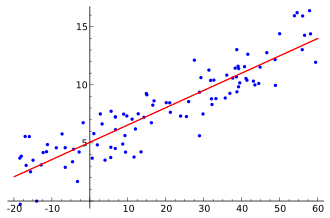
\includegraphics[width=0.6\textwidth]{png/linear_regression.png}
    \caption{线性回归示意图}
    {图源: \uhref{https://en.wikipedia.org/wiki/Linear_regression}{Wikipedia}}
    \label{fig:linear_regression}
\end{figure}

虽然线性回归的名字叫做“回归”,但是事实上我更喜欢叫做线性拟合。它的目的是找到一条直线尽可能“贴近”数据点。在这一基础上,我们可以发现数据之间的规律,从而做出一些预测。不过这里有几个问题:
\begin{itemize}
    \item 为什么要用直线?为什么不用曲线?
    \item 为什么要用直线拟合数据点?这有什么用?
    \item “贴近”数据点的标准是什么?为什么要选择这个标准?
\end{itemize}

我认为用直线的原因无非两点:一是直线 $y = kx+b$ 简单且意义明确,又能处理不少的问题。几何上直线作为基本对象,尺子就能画出;代数上只需要加减乘除,一次函数我们也很早就学过了。而它的思想一路贯穿到了微积分的导数并拓宽到了线性代数。二是许多曲线的回归可以转为线性回归(见后文)。例如指数型的 $y = k \mathrm{e}^{\alpha x}$ 取对数变为 $z = \alpha x + \ln k$,又如分式型的 $y = (\alpha x + \beta)^{-1}$ 换元转化为 $z = \alpha x + \beta$,从而归结为线性拟合。因此带着线性拟合经验再去考虑曲线会更轻松。

至于其意义:一是找到数据的规律,二是做出预测。拟合的系数可以用于测算数据之间的关系,斜率 $k$ 表明输出对输入的敏感程度。最经典的例子莫过于广告投放的边际效应,在一定范围内拟合收益与投入的关系,可以估算当前的边际效益\footnote{边际效益:经济学概念,每增加单位投入,产出会增加多少单位},从而决定是否继续投放。而物理上,比值定义法定义的各种物理量,如电阻、电容等,最常用的测算方式都是线性拟合。例如测量电源输出的若干组电压和电流数据,并拟合出直线,斜率的绝对值是电源的内阻,同时截距顺带给出了电源的电动势,这样测得的数据就可以用于预测电源的输出情况。对我们所处的世界有定量的认识是科学的基础。可测量的数据和数学模型来描述、解释和预测自然现象是科学的基本方法,也是我们拟合的根本目的。

既然有了基本思路,那么如何选择“贴近”的标准呢?直接去度量一堆散点和直线的接近程度多少有点霰弹枪\footnote{霰弹枪:一种枪,射出的子弹像雨点一样散开}打移动靶的感觉,但是我们总是可以计算子弹打到了几环。换言之,两个相差的部分才是关键的,残差的概念由此产生。取出每个点实际值和拟合值的差,就得到了这样一个列表(其中预测值 $\hat y_i = kx_i + b$):
\[
    [r_1, r_2, \ldots, r_n] = [y_1 - \hat y_1, y_2 - \hat y_2, \ldots, y_n - \hat y_n]
\]
度量数据点与直线间偏差这一问题就转为了度量残差与 0 的偏差。还记得勾股定理吗?直角坐标系内一点到 0 的距离是坐标平方和的平方根,只不过这里残差列表是个 $n$ 维的向量,度量它偏离原点的程度就是向量的模。这个模越小,说明拟合的效果越好。这样我们就自然地引入了度量拟合效果的量化标准,不过实际应用中出于方便(特别是计算上的方便),我们通常省去开根号的一步,直接采用残差的平方和,此外还会除以样本点数得到“平均”的残差平方。习惯上称之为\textbf{均方误差}(Mean Squared Error, MSE):
\[
    \text{MSE} = \frac1n |r|^2 = \frac1n \sum_{i=1}^n r_i^2
\]

在踏出下一步之前,我想这里有一点点思考的空间。例如:
\begin{itemize}
    \item 为什么要用平方和而不是直接相加呢?

          这是因为直接相加会有正负相互抵消的可能,度量出的偏差为 0 甚至为负实在是不合理,因此至少要保证每一项都是正数。但是这又引出下一个问题。

    \item 为什么不用绝对值呢?绝对值也是正的啊。

          从高斯分布的角度看,选用平方和自有它的\uhref{https://www.zhihu.com/question/20447622/answer/25186207}{道理}。但是即使读者并不熟悉这些统计的背景,也可以从另一个角度理解:平方和的确是一个更好的度量方式,因为它对大的偏差更加敏感。例如一个残差为 2 的点和一个残差为 4 的点,直接绝对值相加的话是 6,在这里残差为 4 的点贡献了 $4 / 6 \approx 66.7\%$ 的偏差。而它们的平方和是 $2^2 + 4^2 = 20$,残差为 4 的点贡献提升到了 $4^2 / 20 = 80\%$,更加凸显出了 4 的偏差,反映了我们更“关注”它的想法,更符合我们对“偏差”的直观认识。

    \item 为什么要除以样本点数 $n$ 呢?

          一方面是为了跨数据集比较,数据集的大小通常有区别,就像买东西的重量。这正如不能光看价格不看质量就评价 5 元 2 斤的苹果贵还是 3 元 1 斤的苹果贵,我们需要一个“单位”来衡量。另一方面,看完下一个问题你就会明白其中的精妙之处。

    \item 我们直接把所有的残差平方加了起来,但如果有的点重要一些怎么办?

          先说明一下这样的需求并非空想,有时测量条件决定了不同点的可靠性并不相同。以一个精度 1\% 的表为例,测量得到 1.00, 2.00, 3.00 时它们本身允许的误差分别是 0.01, 0.02, 0.03,而非相同。也就是说我们会觉得 1.00 的测量值从残差的大小上\footnote{残差的大小:严谨的说称作绝对误差}更为可靠,这时我们似乎应该衡量一下点的“重要性”。如果你想说一个点很重要怎么办?直观上来讲你可能会想把它重复几遍,例如如果你很关心 $r_1$,你可能会想,这还不简单吗?在误差列表中把 $r_1$ 重复 3 遍就好,就像这样:
          \[
              r = [r_1, r_1, r_1, r_2, r_3, \ldots, r_n]
          \]
          这时再计算均方误差呢,变成了 $n+2$ 个点,一种我们设想中“改善的”均方误差公式就变成了这样:
          \[
              \text{Refined MSE} = \frac1{n+2} \left(2r_1^2 + \sum_{i=1}^{n+2} r_i^2\right)
          \]
          只不过这样的方式无疑有点“笨重”,再仔细想想呢?如果我们把 $1/(n+2)$ 乘到每一项上,就像这样:
          \[
              \text{Refined MSE} = \frac3{n+2} r_1^2 + \frac1{n+2} r_2^2 + \cdots + \frac1{n+2} r_{n+2}^2
          \]
          再对照着上面的列表看一看,$3/(n+2)$ 不正好表明在大小为 $n+2$ 的列表中 $r_1$ 出现了 3 此吗?频次就这样和系数(权重)联系起来了。我们也没必要守着重复 3 次或者 5 次这种固定的规则——至少自然可没有限制重要性之间的比例刚好是整数。这样一来只需要一个权重列表就可以了,权重乘在残差平方前,这就引出了\textbf{加权误差},大权重表示更重要,略微改写一下公式得到:
          \[
              \text{Weighted MSE} = \sum_{i=1}^n w_i r_i^2
          \]
          这里为了方便起见,我们假设权重的和为 1,即 $\sum_{i=1}^n w_i = 1$,如果不为 1,可以先计算误差再除以权重的和。由此可以根据实际情况调整不同点的重要性,也可以看出,之前的均方误差不过是因为在 $n$ 个数中每个残差变量都出现了 1 次,所以权重都设为了 $1/n$。在重要性可变时,加权均方误差无疑提供了一种更加“通用”的度量方式。
\end{itemize}

使用的工具已经准备好了,目标也已经明确了,那么可以开始拟合了。当然,为了简单起见,我们还是只考虑无权重的情况。我们要做的是找到一组参数 $k, b$ 使得均方误差最小,从这一点可以窥见贯穿整个机器学习的核心思想——最小化损失(误差)。形式上,我们会这么写:
\[
    k, b = \argmin_{k, b} \text{MSE} = \argmin_{k, b} \frac1n \sum_{i=1}^n (y_i - kx_i - b)^2
\]
但是它并没有那么神秘:$\arg$ 是 argument 的缩写,是参数的意思。$\min$ 是 minimum 的意思,即最小值。上面的式子完全可以读作“找到 $k, b$ 使得均方误差最小”。虽然项很多,但这本是上只是一个二次函数,所以无论是配方法、对 $k, b$ 分别求导还是使用矩阵方法,都可以很容易地求解。不过我很喜欢另一个较少被人提及的视角——从线性代数和几何的角度来看待这个问题。我们回头看看残差的表达式:
\[
    \begin{aligned}
        r & = [r_1, r_2, \ldots, r_n]                                                     \\
          & = [y_1 - (kx_1 + b), y_2 - (kx_2 + b), \ldots, y_n - (kx_n + b)]              \\
          & = [y_1, y_2, \ldots, y_n] - (k [x_1, x_2, \ldots, x_n] + b [1, 1, \ldots, 1]) \\
    \end{aligned}
\]
我们暂时用一个这样的记号,记 $X^0 = [1, 1, \ldots, 1]$,$X^1 = [x_1, x_2, \ldots, x_n]$,$Y = [y_1, y_2, \ldots, y_n]$,那么残差就可以写成 $r = Y - (kX^1 + bX^0)$。这样一来,我们的目标是找到 $k, b$ 使得 $r$ 的模最小。写到这里,从代数上看可能依然不够直观,让我们换个角度看看。

\begin{figure}[H]
    \centering
    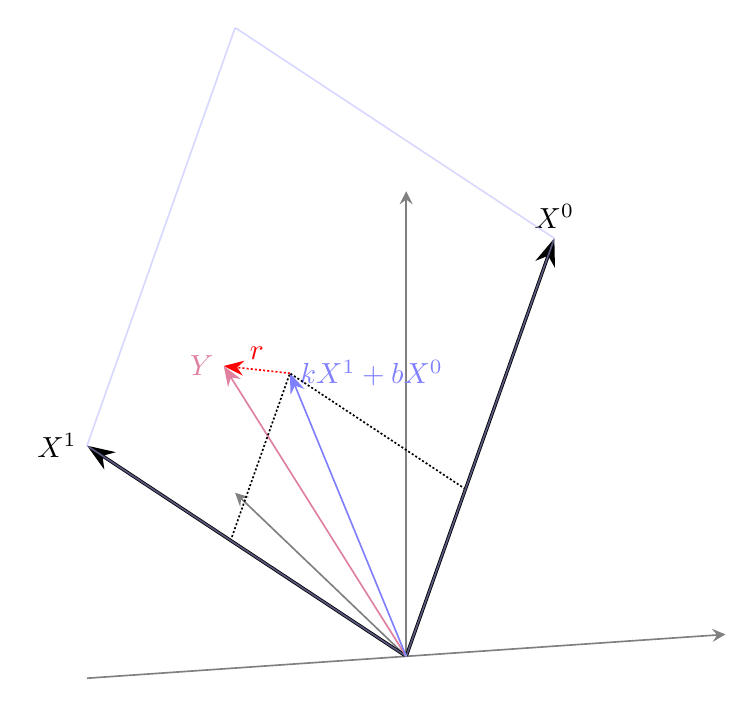
\begin{tikzpicture}[>=Stealth, scale=1.5]
        \begin{axis}[
                view={-15}{20},      % 设置视角 (方位角, 俯仰角)
                axis lines=center,  % 轴从原点开始
                enlargelimits=false,
                ticks=none,         % 取消刻度
                colormap/viridis,
                axis line style={draw=gray},
                % xlabel={$x$},
                % ylabel={$y$},
                % zlabel={$z$}
            ]

            \coordinate (O) at (axis cs:0,0,0);
            \coordinate (Y) at (axis cs:-0.25, 0.6, 0.85);
            \coordinate (A) at (axis cs:-0.15, 0.4, 0.95);

            \addplot3[thick, ->] coordinates {(0,0,0) (1,1,1)} ;
            \node[above, scale=0.7] at (axis cs:1,1,1) {$X^0$};

            \addplot3[thick, ->] coordinates {(0,0,0) (-1,0,1)};
            \node[left, scale=0.7] at (axis cs:-1,0,1) {$X^1$};

            \addplot3[thin, purple!50, ->] coordinates {(0,0,0) (-0.25, 0.6, 0.85)};
            \node[left, purple!50, scale=0.7] at (Y) {$Y$};

            \addplot3[thin, blue!50, ->] coordinates {(0,0,0) (-0.15, 0.4, 0.95)};
            \node[right, blue!50, scale=0.7] at (A) {$kX^1 + bX^0$};

            \addplot3[red, dash pattern=on 0.5pt off 0.5pt, ->] coordinates {(-0.15,0.4,0.95) (-0.25, 0.6, 0.85)};
            \node[red, above, scale=0.7] at (axis cs:-0.2, 0.5, 0.9) {$r$};

            \addplot3[thin, dash pattern=on 0.5pt off 0.5pt] coordinates {(0.4, 0.4, 0.4) (-0.15, 0.4, 0.95) (-0.55, 0, 0.55)};

            \addplot3[surf, color=blue!30, fill=blue!30, shader=flat, opacity=0.5]
            coordinates {(0,1,2) (1,1,1) (0,0,0) (-1,0,1) (0,1,2)};
        \end{axis}
    \end{tikzpicture}
    \caption{从几何的角度看残差}
\end{figure}

从几何上,$kX^1 + bX^0$ 落在它们所处的平面上,求 $r = Y - (kX^1 + bX^0)$ 的最小值实际上就是从点向平面做垂线并求垂线长。平面上的点恰好表示了那些可以精准拟合的数据,而偏离平面的部分则暗示了无论怎么用直线拟合都会有误差。不得不说从几何上看确实清晰很多,事实上也有人从几何角度给出了\uhref{https://www.bilibili.com/video/BV15zPBevERL}{推导},不过掠过这些细节,仅保留一个直观的印象也无大碍。本节的几篇推荐阅读中都用不同的方法解答了如何最小化误差,有详细的推导,因此这里不再赘述。但是我认为如果读者有一些基础的统计知识而且想记住线性回归推导出的结果,那么结论值得一提,不过跳过也无妨。计算出来的结论是这样的:

首先要计算的是样本中心点,对 $b$ 的导数项为 0 推出最优的直线必然经过样本中心点 $(\bar x, \bar y)$,其中
\[
    \bar x = \frac1n \sum_{i=1}^n x_i, \bar y = \frac1n \sum_{i=1}^n y_i
\]
即均值。

看斜率之前先看看方差和协方差,方差\footnote{此注释写给学过数理统计的读者:此处并非样本方差,样本方差除以的是 $n-1$}的表达式是
\[
    \text{Var}(x) = \frac1n \sum_{i=1}^n (x_i - \bar x)^2
\]
是不是感觉很熟悉?这不就是自变量相对均值的 MSE 吗?而协方差的表达式是
\[
    \text{Cov}(x, y) = \frac1n \sum_{i=1}^n (x_i - \bar x)(y_i - \bar y)
\]
它把方差中的平方项换成了 $x$ 和 $y$ 的交叉项,并由此体现出了相关关系。

接下来计算的是斜率 $k$,它的表达式是
\[
    k = \frac{\sum_{i=1}^n (x_i - \bar x)(y_i - \bar y)}{\sum_{i=1}^n (x_i - \bar x)^2}
\]
看起来有些复杂,但是总结起来其实就是协方差除以自变量的方差,即 $k = \text{Cov}(x, y) / \text{Var}(x)$,如果把协方差看作一种乘法\footnote{此注释写给熟悉线性代数的同学:在\uhref{https://en.wikipedia.org/wiki/Inner_product_space\#Random_variables}{向量空间内积}的意义上这几乎正确},那么 $k = (x\cdot y) / (x\cdot x)$ 看起来确实挺像那么回事的。

这样一来,通过点-斜率式方程就可以得到最优的直线,那么直线拟合就告一段落了。

\begin{tcolorbox}[myrecommendbox, title=推荐阅读, breakable=false]
    \begin{itemize}
        \item 用人话讲明白线性回归LinearRegression - 化简可得的文章 - 知乎\\
              \url{https://zhuanlan.zhihu.com/p/72513104}
        \item 非常详细的线性回归原理讲解 - 小白Horace的文章 - 知乎\\
              \url{https://zhuanlan.zhihu.com/p/488128941}
        \item 机器学习| 算法笔记-线性回归(Linear Regression) - iamwhatiwant的文章 - 知乎\\
              \url{https://zhuanlan.zhihu.com/p/139445419}
    \end{itemize}
\end{tcolorbox}

\newpage

\subsection{多项式拟合}

\begin{figure}[H]
    \centering
    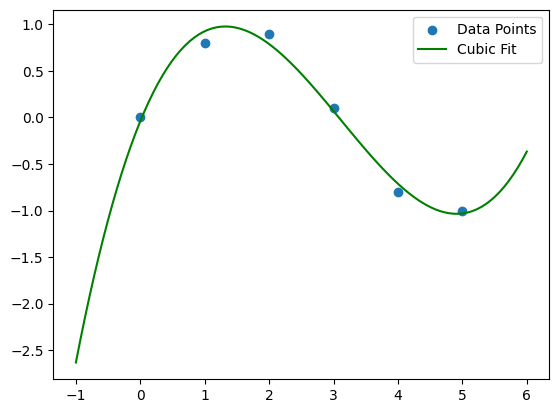
\includegraphics[width=0.6\textwidth]{png/polynomial_fitting.png}
    \caption{多项式拟合示意图(图为 3 次拟合)}
    {图源: \uhref{https://www.geeksforgeeks.org/numpys-polyfit-function-a-comprehensive-guide/}{GeeksforGeeks}}
    \label{fig:polynomial_fitting}
\end{figure}

线性拟合虽然很好,但是如果拿到了明显不线性的一堆数据,那么线性拟合就显得有些力不从心了。不过既然都是拟合,能做一次的那按理来讲也能做多次。多项式拟合就是这样一种思路,只是预测 $\hat y$ 从 $kx+b$ 变成了 $a_0 + a_1 x + \cdots + a_m x^m$\,\footnote{记号说明:虽然习惯上幂次从大到小排列,但是为了下标和幂次的统一性,所以这里选择从常数项到最高次项排列},其中 $m$ 是多项式的次数。而均方误差的表达式甚至几乎不用变,仍然是
\[
    \text{MSE} = \frac1n \sum_{i=1}^n (y_i - \hat y)^2
\]
只不过展开后是一系列的多项式项,待拟合的参数从两个变成了 $m+1$ 个。但是如果观察一下,这个式子仍然是一个(多变量的)二次函数,所以最小化的方法也是一样的。多项式自有多项式的好,能加的项多了,拟合的灵活性也就大了,误差显然会更小。然而与线性拟合相比,它不再有一个可以逐项明确说出意义的解析解,而是只剩下一堆矩阵运算把这些参数算出来。因此形成一个整体上的印象显得尤为重要。

上一小节中,我们从图像看到了这种拟合的几何解释,而多项式拟合也是相似的,还是从 $r$ 的表达式入手
\[
    r = Y - (a_0 X^0 + a_1 X^1 + \cdots + a_m X^m)
\]
对比之前的表达式,当 $a_0, a_1, \ldots, a_m$ 变化时,预测值 $\hat Y = a_0 X^0 + a_1 X^1 + \cdots + a_m X^m$ 也会在一个 $m + 1$ 维的空间中变化,正如之前的平面,这个空间也是一个 $m + 1$ 维的子空间。求最小模的 $r$ 又回到了从点到子空间的垂线问题。虽然我们不得不承认:想象从一个高维的 $n$ 维空间中向 $m+1$ 维的子空间做垂线确实有些困难,但是这多少离我们的几何直觉更近了一些。

系数的意义不那么明确了,但是误差下来了,这是好事吗?也不一定,灵活性的另一面是潜在的\textbf{过拟合}。前文中我们做线性拟合的时候有一个重要的假设是,我们测量的数据带有一定的误差。拟合的直线滤去了大部分的误差,留下了重要的趋势。但是如果灵活性太高,拟合的多项式会过于贴合数据,甚至把误差也拟合进去了。即使在给定的数据上做到了很小的误差,预测新数据的能力却可能会大打折扣。

拿做题打个比方:使用直线拟合明显不线性的数据是方法错了,只能说是没完全学会。但是用接近数据量的参数来拟合数据,留给它的空间都够把结果“背下来”了,捕捉到了数据的细节,却忽略了数据背后的规律,化成了一种只知道背答案的自我感动。在几道例题上能做到滴水不漏,但是一遇到新题就束手无策。

举个例子,在下面这个数据集上试图拟合,我们在二次函数 $y = 0.25 x^2 - x + 1$ 上添加了标准正态分布的噪声,即实际上 $y = 0.25 x^2 - x + 1 + \mathcal{N}(0, 1)$ \footnote{$\mathcal{N}(0, 1)$:表示一个服从\uhref{https://baike.baidu.com/item/\%E6\%A0\%87\%E5\%87\%86\%E6\%AD\%A3\%E6\%80\%81\%E5\%88\%86\%E5\%B8\%83}{标准正态分布}的变量,均值为 0,方差为 1}。
\begin{figure}[h]
    \centering
    \begin{tikzpicture}
        \begin{axis}[
                axis lines=middle,
                xlabel={$x$}, ylabel={$y$},
                grid=major,
                legend pos=north west
            ]
            \addplot[
                only marks,
                mark=*,
                color=blue
            ]
            coordinates {
                    (0.0, 0.423) (0.1, -0.726) (0.2, 1.96) (0.3, 0.065) (0.4, -0.355) (0.5, 0.45) (0.6, -0.778) (0.7, 0.123) (0.8, 0.531) (0.9, -1.097) (1.0, 1.218) (1.1, -0.018) (1.2, 0.363) (1.3, -2.308) (1.4, -0.688) (1.5, 0.5) (1.6, 1.28) (1.7, -0.052) (1.8, 0.45) (1.9, -0.398) (2.0, 0.207) (2.1, 0.237) (2.2, -1.486) (2.3, 0.244) (2.4, -0.215) (2.5, -0.849) (2.6, 0.395) (2.7, -0.185) (2.8, -0.415) (2.9, -0.477) (3.0, 1.11) (3.1, -0.435) (3.2, 0.833) (3.3, 1.451) (3.4, 0.147) (3.5, 0.139) (3.6, -1.163) (3.7, 3.425) (3.8, -0.117) (3.9, 2.428) (4.0, 1.964) (4.1, 1.613) (4.2, 0.992) (4.3, 0.949) (4.4, 1.707) (4.5, 2.736) (4.6, 0.905) (4.7, 1.117) (4.8, 3.352) (4.9, 3.162) (5.0, 2.226) (5.1, 3.536) (5.2, 1.403) (5.3, 2.448) (5.4, 2.652) (5.5, 3.959) (5.6, 3.705) (5.7, 3.537) (5.8, 3.656) (5.9, 4.784) (6.0, 3.247) (6.1, 4.589) (6.2, 2.857) (6.3, 4.194) (6.4, 4.053) (6.5, 2.536) (6.6, 5.568) (6.7, 5.73) (6.8, 3.667) (6.9, 6.415) (7.0, 4.927) (7.1, 5.545) (7.2, 6.754) (7.3, 6.447) (7.4, 7.352) (7.5, 7.55) (7.6, 8.649) (7.7, 7.145) (7.8, 7.837) (7.9, 7.964) (8.0, 9.074) (8.1, 8.135) (8.2, 10.401) (8.3, 8.005) (8.4, 10.431) (8.5, 10.629) (8.6, 8.624) (8.7, 10.726) (8.8, 13.097) (8.9, 12.136) (9.0, 12.849) (9.1, 10.127) (9.2, 14.107) (9.3, 13.364) (9.4, 14.538) (9.5, 12.474) (9.6, 15.591) (9.7, 13.714) (9.8, 16.952) (9.9, 16.317) (10.0, 16.764)
                };
            \addlegendentry{带噪声数据}
            \addplot[
                domain=0:10,
                samples=100,
                color=red,
                thick
            ] {0.25 * x^2 - x + 1};
            \addlegendentry{真实曲线}
        \end{axis}
    \end{tikzpicture}
\end{figure}

那么现在我们来试试用不同次数的多项式拟合这个数据集。我们发现线性拟合还是差不少,因为它没能提供可以制造数据“弯曲”形状的项,2 次曲线的效果几乎和真实曲线一样,即使提升到 3 次也没有太明显的改变。
\begin{figure}[H]
    \centering
    \begin{tikzpicture}
        \begin{axis}[
                axis lines=middle,
                xlabel={$x$}, ylabel={$y$},
                grid=major,
                legend pos=north west
            ]
            \addplot[
                only marks,
                mark=*,
                color=blue
            ]
            coordinates {
                    (0.0, 0.423) (0.1, -0.726) (0.2, 1.96) (0.3, 0.065) (0.4, -0.355) (0.5, 0.45) (0.6, -0.778) (0.7, 0.123) (0.8, 0.531) (0.9, -1.097) (1.0, 1.218) (1.1, -0.018) (1.2, 0.363) (1.3, -2.308) (1.4, -0.688) (1.5, 0.5) (1.6, 1.28) (1.7, -0.052) (1.8, 0.45) (1.9, -0.398) (2.0, 0.207) (2.1, 0.237) (2.2, -1.486) (2.3, 0.244) (2.4, -0.215) (2.5, -0.849) (2.6, 0.395) (2.7, -0.185) (2.8, -0.415) (2.9, -0.477) (3.0, 1.11) (3.1, -0.435) (3.2, 0.833) (3.3, 1.451) (3.4, 0.147) (3.5, 0.139) (3.6, -1.163) (3.7, 3.425) (3.8, -0.117) (3.9, 2.428) (4.0, 1.964) (4.1, 1.613) (4.2, 0.992) (4.3, 0.949) (4.4, 1.707) (4.5, 2.736) (4.6, 0.905) (4.7, 1.117) (4.8, 3.352) (4.9, 3.162) (5.0, 2.226) (5.1, 3.536) (5.2, 1.403) (5.3, 2.448) (5.4, 2.652) (5.5, 3.959) (5.6, 3.705) (5.7, 3.537) (5.8, 3.656) (5.9, 4.784) (6.0, 3.247) (6.1, 4.589) (6.2, 2.857) (6.3, 4.194) (6.4, 4.053) (6.5, 2.536) (6.6, 5.568) (6.7, 5.73) (6.8, 3.667) (6.9, 6.415) (7.0, 4.927) (7.1, 5.545) (7.2, 6.754) (7.3, 6.447) (7.4, 7.352) (7.5, 7.55) (7.6, 8.649) (7.7, 7.145) (7.8, 7.837) (7.9, 7.964) (8.0, 9.074) (8.1, 8.135) (8.2, 10.401) (8.3, 8.005) (8.4, 10.431) (8.5, 10.629) (8.6, 8.624) (8.7, 10.726) (8.8, 13.097) (8.9, 12.136) (9.0, 12.849) (9.1, 10.127) (9.2, 14.107) (9.3, 13.364) (9.4, 14.538) (9.5, 12.474) (9.6, 15.591) (9.7, 13.714) (9.8, 16.952) (9.9, 16.317) (10.0, 16.764)
                };
            \addlegendentry{带噪声数据}

            \addplot[
                domain=0:10,
                samples=100,
                color=red,
                thick
            ] {0.25 * x^2 - x + 1};
            \addlegendentry{真实曲线}

            \addplot[
                domain=0:10,
                samples=100,
                color=orange,
                thick
            ] {1.5142676761793825 * x -3.3366750145602806};
            \addlegendentry{线性拟合}

            \addplot[
                domain=0:10,
                samples=100,
                color=yellow,
                thick
            ] {0.24383409557403493 * x^2 -0.9240732795609664 * x + 0.6865875624112963};
            \addlegendentry{二次拟合}

            \addplot[
                domain=0:10,
                samples=100,
                color=green,
                thick
            ] {0.012628009463763832 * x^3 + 0.054413953617577414 * x^2 -0.17015585855533788 * x + 0.07400282332411103};
            \addlegendentry{三次拟合}
        \end{axis}
    \end{tikzpicture}
\end{figure}

但是如果我们继续增加次数呢?先来看看十次的拟合效果。
\begin{figure}[H]
    \centering
    \begin{tikzpicture}
        \begin{axis}[
                axis lines=middle,
                xlabel={$x$}, ylabel={$y$},
                grid=major,
                legend pos=north west
            ]
            \addplot[
                only marks,
                mark=*,
                color=blue
            ]
            coordinates {
                    (0.0, 0.423) (0.1, -0.726) (0.2, 1.96) (0.3, 0.065) (0.4, -0.355) (0.5, 0.45) (0.6, -0.778) (0.7, 0.123) (0.8, 0.531) (0.9, -1.097) (1.0, 1.218) (1.1, -0.018) (1.2, 0.363) (1.3, -2.308) (1.4, -0.688) (1.5, 0.5) (1.6, 1.28) (1.7, -0.052) (1.8, 0.45) (1.9, -0.398) (2.0, 0.207) (2.1, 0.237) (2.2, -1.486) (2.3, 0.244) (2.4, -0.215) (2.5, -0.849) (2.6, 0.395) (2.7, -0.185) (2.8, -0.415) (2.9, -0.477) (3.0, 1.11) (3.1, -0.435) (3.2, 0.833) (3.3, 1.451) (3.4, 0.147) (3.5, 0.139) (3.6, -1.163) (3.7, 3.425) (3.8, -0.117) (3.9, 2.428) (4.0, 1.964) (4.1, 1.613) (4.2, 0.992) (4.3, 0.949) (4.4, 1.707) (4.5, 2.736) (4.6, 0.905) (4.7, 1.117) (4.8, 3.352) (4.9, 3.162) (5.0, 2.226) (5.1, 3.536) (5.2, 1.403) (5.3, 2.448) (5.4, 2.652) (5.5, 3.959) (5.6, 3.705) (5.7, 3.537) (5.8, 3.656) (5.9, 4.784) (6.0, 3.247) (6.1, 4.589) (6.2, 2.857) (6.3, 4.194) (6.4, 4.053) (6.5, 2.536) (6.6, 5.568) (6.7, 5.73) (6.8, 3.667) (6.9, 6.415) (7.0, 4.927) (7.1, 5.545) (7.2, 6.754) (7.3, 6.447) (7.4, 7.352) (7.5, 7.55) (7.6, 8.649) (7.7, 7.145) (7.8, 7.837) (7.9, 7.964) (8.0, 9.074) (8.1, 8.135) (8.2, 10.401) (8.3, 8.005) (8.4, 10.431) (8.5, 10.629) (8.6, 8.624) (8.7, 10.726) (8.8, 13.097) (8.9, 12.136) (9.0, 12.849) (9.1, 10.127) (9.2, 14.107) (9.3, 13.364) (9.4, 14.538) (9.5, 12.474) (9.6, 15.591) (9.7, 13.714) (9.8, 16.952) (9.9, 16.317) (10.0, 16.764)
                };
            \addlegendentry{带噪声数据}

            \addplot[
                domain=0:10,
                samples=100,
                color=red,
                thick
            ] {0.25 * x^2 - x + 1};
            \addlegendentry{真实曲线}

            \addplot[
                domain=0:10,
                samples=100,
                color=orange,
                thick
            ] {-0.000004129005667 * x^10 + 0.000200033877258 * x^9 - 0.004061827595427 * x^8 + 0.044810202155712 * x^7 - 0.291097682876070 * x^6 + 1.129425113256322 * x^5 - 2.542208192992861 * x^4 + 3.091776048493755 * x^3 - 1.584353162512058 * x^2 - 0.267618886184698 * x + 0.362912675589959};
            \addlegendentry{十次拟合}
        \end{axis}
    \end{tikzpicture}
\end{figure}

你可能会想,虽然是稍微歪了一点,不过这看起来还行吧。但是如果你把 $x$ 的范围稍微扩大一点,你就会发现势头完全不对了。
\begin{figure}[H]
    \centering
    \begin{tikzpicture}
        \begin{axis}[
                axis lines=middle,
                xlabel={$x$}, ylabel={$y$},
                grid=major,
                legend pos=south east
            ]
            \addplot[
                only marks,
                mark=*,
                color=blue
            ]
            coordinates {
                    (0.0, 0.423) (0.1, -0.726) (0.2, 1.96) (0.3, 0.065) (0.4, -0.355) (0.5, 0.45) (0.6, -0.778) (0.7, 0.123) (0.8, 0.531) (0.9, -1.097) (1.0, 1.218) (1.1, -0.018) (1.2, 0.363) (1.3, -2.308) (1.4, -0.688) (1.5, 0.5) (1.6, 1.28) (1.7, -0.052) (1.8, 0.45) (1.9, -0.398) (2.0, 0.207) (2.1, 0.237) (2.2, -1.486) (2.3, 0.244) (2.4, -0.215) (2.5, -0.849) (2.6, 0.395) (2.7, -0.185) (2.8, -0.415) (2.9, -0.477) (3.0, 1.11) (3.1, -0.435) (3.2, 0.833) (3.3, 1.451) (3.4, 0.147) (3.5, 0.139) (3.6, -1.163) (3.7, 3.425) (3.8, -0.117) (3.9, 2.428) (4.0, 1.964) (4.1, 1.613) (4.2, 0.992) (4.3, 0.949) (4.4, 1.707) (4.5, 2.736) (4.6, 0.905) (4.7, 1.117) (4.8, 3.352) (4.9, 3.162) (5.0, 2.226) (5.1, 3.536) (5.2, 1.403) (5.3, 2.448) (5.4, 2.652) (5.5, 3.959) (5.6, 3.705) (5.7, 3.537) (5.8, 3.656) (5.9, 4.784) (6.0, 3.247) (6.1, 4.589) (6.2, 2.857) (6.3, 4.194) (6.4, 4.053) (6.5, 2.536) (6.6, 5.568) (6.7, 5.73) (6.8, 3.667) (6.9, 6.415) (7.0, 4.927) (7.1, 5.545) (7.2, 6.754) (7.3, 6.447) (7.4, 7.352) (7.5, 7.55) (7.6, 8.649) (7.7, 7.145) (7.8, 7.837) (7.9, 7.964) (8.0, 9.074) (8.1, 8.135) (8.2, 10.401) (8.3, 8.005) (8.4, 10.431) (8.5, 10.629) (8.6, 8.624) (8.7, 10.726) (8.8, 13.097) (8.9, 12.136) (9.0, 12.849) (9.1, 10.127) (9.2, 14.107) (9.3, 13.364) (9.4, 14.538) (9.5, 12.474) (9.6, 15.591) (9.7, 13.714) (9.8, 16.952) (9.9, 16.317) (10.0, 16.764)
                };
            \addlegendentry{带噪声数据}

            \addplot[
                domain=-1.5:11.5,
                samples=100,
                color=red,
                thick
            ] {0.25 * x^2 - x + 1};
            \addlegendentry{真实曲线}

            \addplot[
                domain=-1.5: 11.5,
                samples=100,
                color=orange,
                thick
            ] {(((((((((-0.000004129005667 * x + 0.000200033877258) * x - 0.004061827595427) * x + 0.044810202155712) * x - 0.291097682876070) * x + 1.129425113256322) * x - 2.542208192992861) * x + 3.091776048493755) * x - 1.584353162512058) * x - 0.267618886184698) * x + 0.362912675589959};
            \addlegendentry{十次拟合}
        \end{axis}
    \end{tikzpicture}
\end{figure}

一旦离开了拟合的区域,十次拟合的曲线就直勾勾地弯向无穷远,这是因为它把噪声也拟合进去了,从而给出了泛化性\footnote{泛化性:预测原有数据集以外点的能力}极差的结果。这就是过拟合的危害。因为参数量与样本点数量并没有非常显著的差别(10 个参数,100 个样本点),所以从去噪声的角度看,结果过拟合并不奇怪——过滤掉噪声需要更多的数据。

当然解决办法并不是没有,要解决问题先要找到问题的根源。既然得到的函数行为不符合预期,那么很自然地我们会想问,这个函数的系数怎么样呢?在上面这个具体的例子中,函数的表达式是
\[
    \begin{aligned}
        \hat y & = -0.000004129005667 x^{10} + 0.000200033877258 x^9 - 0.004061827595427 x^8   \\
               & \quad + 0.044810202155712 x^7 - 0.291097682876070 x^6 + 1.129425113256322 x^5 \\
               & \quad - 2.542208192992861 x^4 + 3.091776048493755 x^3 - 1.584353162512058 x^2 \\
               & \quad - 0.267618886184698 x + 0.362912675589959
    \end{aligned}
\]

简单估算一下就会发现,例如 3, 4 次项的系数都在个位数级别,再乘以 $x$ 的 3 次方、4 次方数值就会变得很大。10 次方项的系数看起来只有 $4.1\times 10^{-6}$,但是乘上 $x$ 最大值的 10 次方,也就是 $10^{10}$ 后,这个数值同样会飙升到上万的级别。一堆上万级别的数加在一起,倒不如说顶着舍入误差\footnote{舍入误差:就像手动计算时保留几位小数一样,计算机计算的并不是“实数”,而是具有一定精度的浮点数,同样也有误差。例如对于 32-bit 的浮点数,只能精确到 7 个十进制位,这意味着从万位向后数到第 7 位,从百分位就可能已经不准确,在此之后的数位就不太可靠了。}还能够回归到原来的数据集上已经是奇迹了。也就只有 MSE 可以限制一下它在数据集内的行为,出了预定义的范围,这个高次函数大概就放飞自我了。

不过如果一定要用高次函数,补救的办法也不是没有。既然这些系数导致了很大的数值,那限制一下这些数值就好了,这就是\textbf{正则化}的思路。我们在待优化的函数上加上一个惩罚项,同样地使用平方求和的形式,只不过这次是对系数进行惩罚,为了让系数尽量小,即尽量贴近于 $0$,自然想到把它们的平方也加起来(再乘以一个权重),优化的目标\footnote{Loss:损失,与前文单纯使用 MSE 时相同,我们希望让它尽可能小,它的每一项包含了我们对拟合结果的一个美好“祝愿”,MSE 项希望它误差减小,正则化项希望它系数正常。}变成了
\[
    \text{Loss} = \text{MSE} + \underset{\text{正则化项}}{\underbrace{\lambda \sum_{i=1}^{10} a_i^2}}
\]
可调参数 $\lambda$ 表明我们希望在多大程度上抑制系数。然而这里存在一个致命的问题,不同系数对最终结果的影响不同,例如在 $x=10$ 这一点上,$x^{10}$ 项的系数对结果的影响远远大于 $x$ 项的系数,即使是 $4.1\times 10^{-6}$ 这样微小的 $10$ 次项系数也会导致非常大的数值。平方后这一系数变得十分微小,原本用于约束系数大小的正则化项对它的影响更是微乎其微。那么怎么办呢?

再仔细想想问题在哪里,我们发现一路下来导致问题的根源都是 $x$ 的高次项即使在系数很小时也会导致数值爆炸。但是如果我们把 $x$ 放到 $[-1, 1]$ 的闭区间内呢?这样即使是 $x^{10}$ 项,$x$ 的 10 次方也不会超过 $1$,系数再怎么大,至少在小范围内也不会导致数值爆炸,这样一来正则化项才能发挥其约束作用。

操作上只需要把 $[0, 10]$ 范围内的 $x$ 线性地映射到 $[-1, 1]$ 范围内。这很简单,令 $z = 0.2 x - 1$ 再对 $y$ 用 $z$ 的多项式拟合,这种操作称作归一化\footnote{归一化:调整数据到某个给定的范围内,使数据在不同场景下更加可比、更加数值稳定。前文计算误差时取平均实际上也是一种归一化。}。

事实上只需要一个很小的 $\lambda$ 就可以在一定程度上抑制高次项的系数,这里我们取 $\lambda = 0.01$,我们优化的目标变为了
\[
    \text{Loss} = \text{MSE} + 0.01 \sum_{i=1}^{10} a_i^2
\]
这时拟合出来的图像是这样的:

\begin{figure}[H]
    \centering
    \begin{tikzpicture}
        \begin{axis}[
                axis lines=middle,
                xlabel={$z$}, ylabel={$y$},
                grid=major,
                legend pos=north west
            ]
            \addplot[
                only marks,
                mark=*,
                color=blue
            ]
            coordinates {
                    (-1.0, 0.423) (-0.98, -0.726) (-0.96, 1.96) (-0.94, 0.065) (-0.92, -0.355) (-0.9, 0.45) (-0.88, -0.778) (-0.86, 0.123) (-0.84, 0.531) (-0.82, -1.097) (-0.8, 1.218) (-0.78, -0.018) (-0.76, 0.363) (-0.74, -2.308) (-0.72, -0.688) (-0.7, 0.5) (-0.68, 1.28) (-0.66, -0.052) (-0.64, 0.45) (-0.62, -0.398) (-0.6, 0.207) (-0.58, 0.237) (-0.56, -1.486) (-0.54, 0.244) (-0.52, -0.215) (-0.5, -0.849) (-0.48, 0.395) (-0.46, -0.185) (-0.44, -0.415) (-0.42, -0.477) (-0.4, 1.11) (-0.38, -0.435) (-0.36, 0.833) (-0.34, 1.451) (-0.32, 0.147) (-0.3, 0.139) (-0.28, -1.163) (-0.26, 3.425) (-0.24, -0.117) (-0.22, 2.428) (-0.2, 1.964) (-0.18, 1.613) (-0.16, 0.992) (-0.14, 0.949) (-0.12, 1.707) (-0.1, 2.736) (-0.08, 0.905) (-0.06, 1.117) (-0.04, 3.352) (-0.02, 3.162) (0.0, 2.226) (0.02, 3.536) (0.04, 1.403) (0.06, 2.448) (0.08, 2.652) (0.1, 3.959) (0.12, 3.705) (0.14, 3.537) (0.16, 3.656) (0.18, 4.784) (0.2, 3.247) (0.22, 4.589) (0.24, 2.857) (0.26, 4.194) (0.28, 4.053) (0.3, 2.536) (0.32, 5.568) (0.34, 5.73) (0.36, 3.667) (0.38, 6.415) (0.4, 4.927) (0.42, 5.545) (0.44, 6.754) (0.46, 6.447) (0.48, 7.352) (0.5, 7.55) (0.52, 8.649) (0.54, 7.145) (0.56, 7.837) (0.58, 7.964) (0.6, 9.074) (0.62, 8.135) (0.64, 10.401) (0.66, 8.005) (0.68, 10.431) (0.7, 10.629) (0.72, 8.624) (0.74, 10.726) (0.76, 13.097) (0.78, 12.136) (0.8, 12.849) (0.82, 10.127) (0.84, 14.107) (0.86, 13.364) (0.88, 14.538) (0.9, 12.474) (0.92, 15.591) (0.94, 13.714) (0.96, 16.952) (0.98, 16.317) (1.0, 16.764)
                };
            \addlegendentry{带噪声数据}

            \addplot[
                domain=-1.4: 1.4,
                samples=100,
                color=red,
                thick
            ] {0.25 * ((x+1)*5)^2 - (x+1)*5 + 1};
            \addlegendentry{真实曲线}

            \addplot[
                domain=-1.4:1.4,
                samples=100,
                color=orange,
                thick
            ] {0.056914714852145956 * x^10
                -0.16883868373880576 * x^9
                +0.2748227691835253 * x^8
                +0.02818103309527224 * x^7
                +0.8506420254328089 * x^6
                +0.5250028027489858 * x^5
                +1.8635063516688952 * x^4
                +1.8797071938317609 * x^3
                +3.414068726324771 * x^2
                +6.0490130644654645 * x^1
                +2.5048936484111635};
            \addlegendentry{十次拟合}
        \end{axis}
    \end{tikzpicture}
\end{figure}

虽然图中拟合曲线与真值在数据集外确实仍然有显著的差距,但经过自变量归一化和参数正则化项的加入,拟合的曲线至少把数据的大体趋势成功地延伸到了数据集的一个邻域内,不至于像原本的那样惨不忍睹。

不过在实际应用中,几乎不会用到 5 次以上的多项式拟合。仍然是因为容易过拟合:就以 $[-1, 1]$ 上的函数为例,$x^5$ 与 $x^7$ 的图像几乎是一样的,它们最大的差值仅为 0.12,这意味着如果允许的高次项太多,一点点微小的噪声就能让轻易地把五次项的系数“分给”七次项,或者反之。这导致拟合的数值稳定性很差,因此显然不太可靠。因此比起正则化或者归一化,更重要的是,我们应该意识到,高次函数并不是万能的,当你觉得需要用到很高次的函数才能成功时,不如先想想,多项式的假设真的合适吗?

我们注意到一个重要的事实:虽然拟合的参数在变化,但是我们仍然需要人为地设定多项式的次数,正则项(如果有的话)权重也需要人为设定。这些先验的\footnote{先验:在观测到数据之前,我们已经了解了数据的某些特征。}参数通常称为\textbf{超参数}。如何用模型拟合固然是重要的问题,但是模型的结构,包括如何选取适当的超参数也有学问。因为它们通常不是直接从数据中学习的,而需要人为设定。\uhref{https://www.zhihu.com/question/625846838/answer/3251736042}{有道是}“学而不思则欠拟合,思而不学则过拟合”,我们只有在一定程度上了解问题的本质才能做出适当的选择。

\begin{tcolorbox}[myrecommendbox, title=推荐阅读, breakable=false]
    \begin{itemize}
        \item 多项式拟合的介绍与例子 - 姓甚名谁的文章 - 知乎\\
              \url{https://zhuanlan.zhihu.com/p/366870301}
        \item 理科生觉得哪些知识不知道是文科生的遗憾? - 一只小猫咪的回答 - 知乎\\
              \url{https://www.zhihu.com/question/270455074/answer/2374983755}
        \item 人的大脑会不会出现“过拟合”病? - 莲梅莉usamimeri的回答 - 知乎\\
              \url{https://www.zhihu.com/question/625846838/answer/3250463511}
    \end{itemize}
\end{tcolorbox}

\subsection{高维的线性拟合}

\section{逻辑亦数据}
% 从程序执行的视角开始,引入数据是如何编码逻辑的
\subsection{逻辑门}
\subsection{程序是怎么执行起来的}
\subsection{位运算与bit-flag}

\section{神经网络:一个大的函数}
% 从函数拟合的角度引入神经网络
\subsection{知道目标就可以拟合了?}
\subsection{激活函数与非线性}
\subsection{神经网络的训练}
\subsection{如果不知道目标,只知道回报呢?}

\section{泛化性:一个矛盾}
% 从训练集到测试集的泛化性
\subsection{过拟合与欠拟合}
\subsection{网络的大小好像小于训练数据?哪来的泛化性}
\subsection{训练好像被卡住了——香农极限}

\section{你能猜到一句话接下来要说什么?}
% 从信息论的角度引入预测
\subsection{什么是“废话”?}
\subsection{jpeg虽然有损,但为什么说是极其成功的?}
\subsection{熵与压缩}
\subsection{马尔可夫链}

\section{压缩即智能}
% 从压缩的角度引入智能
\subsection{你是如何看出对面的人心情怎么样的?}
\subsection{压缩的极限——区分能力的边界}
\subsection{从母语词汇看对事物的认识}
\subsection{压缩的本质}

\section{潜空间:更适合机器人的编码方式}
% 从压缩的角度引入潜空间
\subsection{潜空间是什么?}
\subsection{高维空间的维数灾难}
\subsection{“空空”的空间的另一面——维数远不是储存能力的极限}

\section{但是,代价是什么:可解释性的地狱}
% 从压缩的角度引入可解释性
\subsection{想想什么是“解释”?}
\subsection{神经网络不能很好地被解释}

\section{再论网络结构} %:全连接、循环神经网络、卷积神经网络、残差链接与transformer}
% 介绍常见的网络结构
\subsection{全连接网络}
\subsection{循环神经网络}
\subsection{卷积神经网络}
\subsection{深度学习与残差链接}
\subsection{transformer}
\subsection{自编码器与扩散模型}
\subsection{仿人的架构——专家模型}

\section{杂谈}
% 一些更有哲学或社会学色彩的问题
\subsection{矩阵式研究——场景与模型的排列组合}
\subsection{AI圈的常见行话}
\subsection{AI——生产力还是毁灭?}
\subsection{新人类与自由意志?}

\end{document}